\documentclass[12pt]{article}
\usepackage{amsmath}
\usepackage{amssymb}
\usepackage[letterpaper,top=1.25in,bottom=1in,left=0.75in,right=0.75in,centering]{geometry}
%\usepackage{fancyhdr}
\usepackage{enumerate}
%\usepackage{lastpage}
\usepackage{multicol}
\usepackage{graphicx}

\reversemarginpar

%\pagestyle{fancy}
%\cfoot{}
%\lhead{Math 1560}\chead{Test \# 1}\rhead{May 18th, 2017}
%\rfoot{Total: 10 points}
%\chead{{\bf Name:}}
\newcommand{\points}[1]{\marginpar{\hspace{24pt}[#1]}}
\newcommand{\skipline}{\vspace{12pt}}
%\renewcommand{\headrulewidth}{0in}
\headheight 30pt

\newcommand{\di}{\displaystyle}
\newcommand{\abs}[1]{\lvert #1\rvert}
\newcommand{\len}[1]{\lVert #1\rVert}
\renewcommand{\i}{\mathbf{i}}
\renewcommand{\j}{\mathbf{j}}
\renewcommand{\k}{\mathbf{k}}
\newcommand{\R}{\mathbb{R}}
\newcommand{\aaa}{\mathbf{a}}
\newcommand{\bbb}{\mathbf{b}}
\newcommand{\ccc}{\mathbf{c}}
\newcommand{\dotp}{\boldsymbol{\cdot}}
\newcommand{\bbm}{\begin{bmatrix}}
\newcommand{\ebm}{\end{bmatrix}}                   
                  
\begin{document}


\author{Instructor: Sean Fitzpatrick}
\thispagestyle{empty}
\vglue1cm
\begin{center}
{\bf MATH 1560 - Tutorial \#8 Solutions}
\end{center}

\textbf{Additional practice problems:}
\begin{enumerate}
\item Find the dimensions of the rectangle of largest area that can be inscribed in an equilateral triangle of side length $L$, if one side of the rectangle must lie along  the base of the triangle.

\begin{multicols}{2}
A diagram of the situation is shown to the right. Note that the rectangle must be centred with respect to the triangle; if not, one corner does not touch the triangle and we have room to make the rectangle wider, so we would not have the largest area. Let us assume that the bottom of the triangle lies along the $x$-axis, with the center at $(0,0)$. Then the bottom-right corner of the triangle is at $(L/2,0)$. If $h$ is the height of the triangle, we have $h^2+(L/2)^2=L^2$, so $h=\frac{\sqrt{3}}{2}L$, putting the top of the triangle at $(0,\sqrt{3}L/2)$.

\columnbreak

\begin{center}
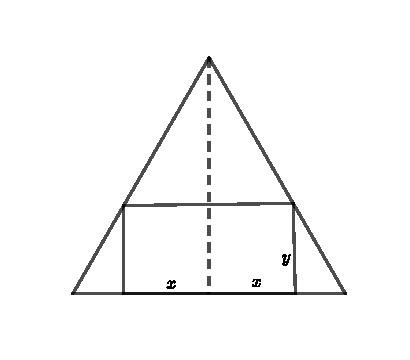
\includegraphics[width=\columnwidth]{Tut8-01sol}
\end{center}
\end{multicols}
The slope of the line joining these two corners is $\dfrac{-\sqrt{3}L/2}{L/2} = -\sqrt{3}$, so the equation of the line (using the intercept $b=\sqrt{3}L/2$) is
\[
y = -\sqrt{3}x+\frac{\sqrt{3}}{2}L.
\]

Now, the base of our rectangle is $2x$, and the height is $y$, so the area is $A=2xy$. The equation of our line gives us $y=-\sqrt{3}x-\sqrt{3}L/2$, so as a function of $x$, the area is
\[
A(x) = 2x\left(-\sqrt{3}x-\frac{\sqrt{3}}{2}L\right)=(\sqrt{3}L)x-2\sqrt{3}x^2, \quad x\in [0,L/2].
\]
(Note that $x$ has to be between $0$ and $L/2$, as per the diagram.) Since $A(0)=0$ and $A(L/2)=0$ (if $x=L/2$, $y=0$), the maximum must occur at a critical number. We find
\[
A'(x) = \sqrt{3}L-4\sqrt{3}x,
\]
so $A'(x)=0$ when $x = \dfrac{\sqrt{3}L}{4\sqrt{3}}=\dfrac{L}{4}$. Thus, the width of the rectangle must be $2x=\dfrac{L}{2}$, and 
\[
y = -\sqrt{3}\cdot\frac{L}{4}+\frac{\sqrt{3}}{2}L = \frac{\sqrt{3}}{4}L.
\]

\item If $1200 \text{ m}^2$ of material are available to make a box with a square base and open top, find the largest possible volume of the box.

The dimensions of our box are $x\times x\times y$, where $x$ is the length of one side of the square base, and $y$ is the height. The volume is therefore $V=x^2y$, and since we are using $1200 \text{ m}^2$ of material, the surface area must satisfy
$x^2+4xy = 1200.$
(The base has area $x^2$ and there are 4 sides of area $xy$.) Using this equation, we can write $y$ in terms of $x$, giving us 
\[
y=\frac{1200}{4x}-\frac{x^2}{4x} = \frac{300}{x}-\frac{x}{4},
\]
and 
\[
V(x) = x^2\left(\frac{300}{x}-\frac{x}{4}\right) = 300x-\frac{x^3}{4}.
\]
In this case we must have $0<x<\sqrt{1200}$, and if we approach either extreme, we see that the volume goes to zero, so the maximum must occur at a critical number. We find
\[
V'(x) = 300-\frac{3x^2}{4} = \frac{1200-3x^2}{4} =\frac{3}{4}(400-x^2)=\frac{3}{4}(20-x)(20+x).
\]
Thus, $V'(x)=0$ for $x=20$ and $x=-20$. Since we must have $x>0$, we reject $x=-20$, giving us $x=20$, $y=\dfrac{300}{20}-\frac{20}{4}=15-5=10$, so the dimensions are $20\times 20\times 10$.

\textbf{Note:} If we construct the sign diagram for $V'(x)$, we can see that $V'(x)$ changes from positive to negative at $x=20$, confirming that this is a maximum.

\item A farmer wants to fence in an area of 1.5 million square feet in a rectangular field, and then divide the field in half with a fence parallel to one of the sides of the rectangle. How should he do this in order to minimize the cost of the fencing?

Let $x$ and $y$ be the dimensions of the field, with the additional fence parallel to the side of length $x$. Then the area of the field is $A=xy$, and the amount of fencing required is $L=3x+2y$.

Our constraint is that $xy=1500000$, allowing us to write $y=\dfrac{1500000}{x}$, and thus
\[
L(x) = 3x+\frac{3000000}{x}, \text{ with } x>0.
\]
Note that our domain is $(0,\infty)$, and that $L(x)\to\infty$ as $x\to 0$ or $x\to \infty$, so to minimize the amount of fencing, we need to look for a local minimum. We have 
\[
L'(x) = 3-\frac{3000000}{x^2} =\frac{3(x^2-1000000)}{x^2}=\frac{3(x-1000)(x+1000)}{x^2}.
\]
We have $L'(x)=0$ for $x=\pm 1000$, but since $x=-1000$ is not in the domain, only $x=1000$ is a critical number. (We also note that $L'(x)$ changes from negative to positive at $x=1000$, so this is indeed a local minimum.)

The farmer should therefore fence a field with dimensions $1000\times 1500$, with the additional length of fence parallel to the side of length 1000.
\end{enumerate}




\newpage
%\thispagestyle{empty}

\textbf{Assigned problems:}
\begin{enumerate}
\item An animal sanctuary is building a rectangular enclosure to hold adorable bunnies. To save cost, they decide to build the enclosure next to an existing jaguar pen, allowing them to use the fence around the pen for one side of the rabbit enclosure.

Given that the side of the jaguar pen to be shared is 30 m long, and that 50 m of fencing are available for the bunnies, what is the largest area that can be enclosed?

Does your answer change if the side of the jaguar pen is only 20 m long?

\bigskip

Let the dimensions of the pen be $x\times y$, with the side of length $y$ parallel to the existing fence. Since this fence has length 30 m, we must have $0\leq y\leq 30$ to ensure that the new fence does not extend past the old one.

We then have to fence two sides of length $x$ and one of length $y$, for a total of $2x+y=50$ m of fencing. Solving for $y$, we have $y=50-2x$, so the area is given by
\[
A(x)=x(50-2x)=50x-2x^2.
\]
Note that when $y=30$, we have $2x+30=50$, so $x=10$, and when $y=0$, we have $2x=50$, so $x=25$, giving us a domain of $10\leq x\leq 25$.

Note further that $A(10) = 10(30)=300$, and $A(25) = 25(0)=0$ for the values at the endpoints of our domain. Looking for critical values, we find
\[
A'(x)= 50-4x=0 \text{ for } x = 50/4 = 12.5 \text{ m}.
\]
Since $12.5\in [10,25]$, this is a critical number, and we compute
\[
A(12.5) = 12.5(25) = 312.5,
\]
which is our maximum area.
\newpage

\item A fugitive from the law is attempting to reach his accomplice, who is waiting in an escape vehicle (a beige 1992 Ford Aerostar minivan) on the far side of a river.

The river is 1 km wide, and the van is waiting 5 km downstream from where the fugitive has just jumped into the river. If the fugitive can swim at 3 km/h and run at 9 km/h, how far downstream is the point on the far bank that the fugitive should swim to in order to reach his accomplice as soon as possible?

\bigskip

\begin{multicols}{2}
We diagram the situation on the right. The fugitive begins at point A, and plans to swim to the point C, before running to the point D. We let $x$ be the distance from B to C, so that he must swim a distance of $\sqrt{1+x^2}$.
\columnbreak


\begin{center}
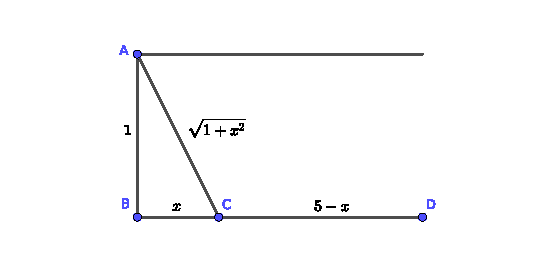
\includegraphics[width=\columnwidth]{Tut8-12sol}
\end{center}
\end{multicols}
The time it takes to make it to the waiting van is given by
\[
t(x) = \frac{\sqrt{1+x^2}}{3}+\frac{5-x}{9}, \quad \text{ for } 0\leq x\leq 5.
\]
Note that $t(0)=\frac13+\frac59=\frac89\approx 0.89$ h, and $t(5) = \frac{\sqrt{26}}{2} \approx 1.7$ h. To find the optimal route, we compute
\[
t'(x) = \frac{x}{3\sqrt{1+x^2}}-\frac19 = \frac{3x-\sqrt{1+x^2}}{9\sqrt{1+x^2}}.
\]
Thus $t'(x)=0$ when $3x=\sqrt{1+x^2}$, or $9x^2=1+x^2$, giving us $x=\dfrac{1}{\sqrt{8}}$ as the desired distance. To confirm, note that
\[
t(1/\sqrt{8}) = \frac{\sqrt{1+1/8}}{3}+\frac{5-1/\sqrt{8}}{9}=\frac59+\frac{\sqrt{8}}{9}\approx 0.87 \text{ h}.
\]
(Frankly, he probably should just swim straight across, since the time saved by landing a distance of $1/\sqrt{8}$ km downstream is less than a minute, which is probably less time than he'd spend solving this problem.)
\end{enumerate}
\newpage

\textbf{Additional exam practice:}
\begin{enumerate}
\item Compute the following derivatives:
\begin{enumerate}
\item $\di\frac{d}{dx}(e^{2x}\tan(x^2)) = 2e^{2x}\tan(x^2)+2xe^{2x}\sec^2(x^2)$



\item $\di\frac{d}{dx}(\sin^3(x^2+5x))=3(2x+5)\sin^2(x^2+5x)\cos(x^2+5x)$

\item $\di\frac{d}{dx}(1+x^2)^x = \frac{d}{dx}e^{x\ln(1+x^2)}=(1+x^2)^x(\ln(1+x^2)+\frac{2x^2}{1+x^2}$

\item $\di \frac{d}{dx}\sin((f(x)^4))=4\cos(f(x)^4)(f(x)^3)f'(x)$

\end{enumerate}

\item Evaluate the following integrals:

\begin{enumerate}
\item $\di \int 2x\sin(x^2)\,dx=\cos(x^2)+C$


\item $\di \int 5\sec^2(5x)e^{\tan(5x)}\,dx=\tan(5x)+C$

\item $\di \int (2e^{2x}\sin(x)+e^{2x}\cos(x))\,dx=e^{2x}\sin(x)+C$

\item $\di \int \frac{1}{x\ln(x)}\,dx=\ln(\abs{\ln(x)})+C$

(The domain of the function being integrated is $(0,1)\cup (1,\infty)$, since we need $x>0$ for $\ln(x)$ to be defined, and $x\neq 1$ to have $\ln(x)\neq 0$. On the right, we don't need an absolute value in the inside logarithm, since we already know $x>0$, but we do need the absolute value around the inside logarithm, since it will be negative for $x\in (0,1)$.)
\item $\di \int \cos(\sin(\sin(\sin(x))))\cos(\sin(\sin(x)))\cos(\sin(x))\cos(x)\,dx = \sin(\sin(\sin(\sin(x))))+C$
\end{enumerate}


\item A helicopter is hovering above a lake when its engine fails. At what altitude was the helicopter hovering, if it hits the water 8 seconds later? Assume acceleration due to gravity is $10 \text{ m/s}^2$ downwards.

If we take $y(t)$ to be the height above the ground (with the upward direction positive) then $y(0)=h$ is the initial height of the helicopter, and $y''(t)=-10$, giving $y'(t)=-10t$ (the initial speed is zero) and $y(t)=h-5t^2$. When $t=8$ we get $y(8)=0=h-320$, so $h=320$ m was the height of the helicopter.

If we take $y(t)$ to be the distance fallen by the helicopter (with downward direction positive), then $y(0)=0$ is the initial distance, and $y''(t) = +10$, giving $y'(t)=10t$ (initial speed is still zero) and $y(t)=5t^2$. Then, we have $y(8)=5(8^2)=320$ as the distance fallen as it hits the water, so again the original height must have been $320$ m.
\newpage


\item Given $\di f(x) = x^3-\frac{3}{x}$,
\begin{enumerate}
\item Solve the equation $f'(x)=0$.

We have $f'(x) = 3x^2+\frac{3}{x^2} = \frac{3(x^4+1)}{x^2}$, which is positive for all values of $x$ except $x=0$, where it is undefined. Thus, there are no solutions to $f'(x)=0$.

\item Find the intervals where $f$ is increasing/decreasing.

By the above, $f$ is increasing on $(-\infty, 0)\cup(0,\infty)$ and decreasing nowhere.

\item Find the coordinates of any local maxima or minima.

There are no local extrema, since there are no critical points.


\item Find the intervals where $f$ is concave up/down.

We have $f''(x) = 6x-\frac{6}{x^3}=\frac{6x^4-6}{x^3}=\frac{6(x-1)(x+1)(x^2+1)}{x^3}$.

If we draw a sign diagram (I've left mine out due to lack of time...) we find that $f''(x)>0$, and hence the graph of $f$ is concave up, on $(-1,0)\cup (1,\infty)$, and $f''(x)<0$, and hence the graph of $f$ is concave down, on $(-\infty, -1)\cup (0,1)$.

\end{enumerate}
\end{enumerate}

\end{document}